\section{The response of a tilted cone}

Repeating the calculation of the response function is now straightforward, but rather tedious.
Due to the boost transformation, the elements of the spinor in the untilted system, Eq. \eqref{eq:34}, mix.
We thus have twice as many terms to keep track of.
\subsection{Explicit form of the matrix elements}

Consider the expression for the current operator, Eq. 4.39, which we derived form the time evolution relation
\[
  \dot{A} = [A, H]/i\hbar,
\]
by considering \(\vec{v} = \vec\dot{r}\), as \(\vec{J} = e \vec{v}\).
In the tilted Hamiltonian, the tilt term thus causes another term in the current operator.
\begin{equation}
  \label{eq:75}
  \begin{split}
    \vec{v} = \vec\dot{r} &= \frac{1}{i \hbar } [\vec{r}, H] \\
    &= \frac{s v_{F} \sigma ^{ i}}{i \hbar } [\vec{r}, p_{i} + e A_{i}] + \frac{1}{i\hbar } [\vec{r}, \omega_{0} \vec{k}]\\
    &= \frac{s v_{F} \sigma ^{ i}}{i \hbar } (i\hbar + e[\vec{r}, A_{i}]) + \vec{\omega}_{0}\\
    &= s v_{F} \sigma ^{i} + \vec{\omega} _{0}.
  \end{split}
\end{equation}

Take for example the matrix element of the current operator
\[
  J_{\vec{k} m s; \vec{k}+\qvec{q} n s } (\vec{q}) = \int \mathrm{d}y e^{-i q_{y} y}
  s v_{F} e \phi ^{*}_{\vec{k} m s} (y) \sigma ^{x} \phi _{\vec{k} + \qvec{q} n s}(y).
\]
We must find the matrix product \(\phi \sigma_{x} \phi \).
Recall that \(\phi = \frac{1}{\mathcal{N}} e^{\theta /2 \sigma _{x}} \tilde{\phi} \), and thus we must find
\[
  \phi ^{*} \sigma _{x} \phi
  = \frac{1}{\mathcal{N}^{*} \mathcal{N}} \tilde{\phi}^{*} e^{\theta /2 \sigma _{x}} \sigma _{x} e^{\theta /2 \sigma _{x}} \tilde{\phi}
  =  \alpha \tilde{\phi}^{*} \sigma _{x} e^{\theta \sigma _{x}} \tilde{\phi}.
\]
With the previously found solution \(\theta = - \tanh ^{-1} t^s_{x}\), we get the rather simple form
\[
  e^{\theta \sigma _{x}} =
  \begin{pmatrix}
    1 & - s t^s_{x}\\
    -s t^s_{x} & 1
  \end{pmatrix}
  \frac{1}{\sqrt{1-t_{x}}}.
\]
With
\begin{equation}\label{eq:76}
  \tilde{\phi} = e^{-\frac{1}{2} \chi ^2}
  \begin{pmatrix}
    a_{\vec{k} m s} H_{M-1} (\chi)\\
    b_{\vec{k} m s} H_{M} (\chi)
  \end{pmatrix}
\end{equation}
we see how the expressions change when \(t^s_{x}\) become non-zero.
Where we previoulsy had
\begin{equation}
  \label{eq:77}
  \tilde{\phi}  ^{*}_{\vec{k} m s} \sigma _{x} \tilde{\phi}  _{\vec{k} + \qvec{q} n s}
  =
  a_{\vec{k} m s} H_{M-1}(\dots) \left[ b_{\vec{k}+\qvec{q} n s} H_{N}(\dots) \right]
  + \dots
\end{equation}
the contents of the square brackets must now include also the other element of the spinor:
\begin{equation}
  \label{eq:78}
  \alpha \tilde{\phi}  ^{*}_{\vec{k} m s} \sigma _{x} e^{\theta \sigma _{x}} \tilde{\phi}  _{\vec{k} + \qvec{q} n s}
  =
  a_{\vec{k} m s} H_{M-1}(\dots)
  \left[
    b_{\vec{k}+\qvec{q} n s} H_{N}(\dots)
    - s t^s_{x} a_{\vec{k} + \qvec{q} n s} H_{N-1} (\dots)
  \right]
  + \dots .
\end{equation}

First of all, let us consider the exponent of the product.
Due to the extra term in \(\chi\), this becomes more elaborate.
The exponent is of course
\begin{equation}
  \label{eq:79}
  \exp\{-i q_{y} y - \frac{1}{2} \chi_{\vec{k}} ^2 - \frac{1}{2} \chi _{\vec{k} + \qvec{q}}^2\}
\end{equation}
A straightforward but tedious calculation shows that the argument of the exponent can be written as
\begin{equation}
  \label{eq:80}
  -\frac{\alpha}{l_{B}^2} \left(y + \frac{l_{B}^2}{2 \alpha } (i q_{y} - (q'_x + 2 k'_x))\right)^2
  -\frac{l_{B}^2}{4 \alpha } (q_{y}^2 + 2i (q'_x + 2 k'_x) q_{y} + ( q' _{x} )^2 ),
\end{equation}
where we have defined
\begin{align}
  \label{eq:qkprime}
  q' _x &= q_x \alpha  - \frac{\beta}{v_{F} }( E^0_{n,\alpha B} - E^0_{m, \alpha B} ),\\
  k' _x &= k_x\alpha - \frac{\beta}{v_F } E^0_{m, \alpha B}.
\end{align}
\todo{check sign of E above}
These must not be confused with the transformed momenta \( \tilde{k} \), which are similar in form.
Eq. \eqref{eq:80} is on the same for as in the untilted cone case, and we may thus proceed with the same method.
Make a change of variable
\[
\tilde{y} = \frac{\sqrt{\alpha }}{l_{B}} \left(y + \frac{l_{B}^2}{2\alpha } (iq_{y} - 2 k' _x - q' _x )\right),
\]
\todo{Follow up the substitution of the root in the integral. Consider moving the root into \(\Xi \)}
to get the exponent on the form \(e^{-\tilde{y}^2}\).
With this substitution,
\begin{align}
  \chi _{\vec{k}} &= \tilde{y} + \frac{l_{B}}{2 \sqrt{\alpha }} \left(q' _x - i q_{y}\right),\\
  \chi _{\vec{k} + \qvec{q}} &= \tilde{y} + \frac{l_{B}}{2 \sqrt{\alpha }} \left(- q' _x - i q_{y}\right).
\end{align}
Doing this, Eq. (4.59) \todo{fix ref} in the project thesis, becomes
\begin{equation}
  \begin{split}
    J_{\vec{k}ms; \vec{k}+\qvec{q} ns}(\vec{q}) &=
    \frac{s v_F e}{\sqrt{\alpha }} \int \mathrm{d}\tilde{y} \: l_B
    \exp \left[
      -\frac{l_{B}^2}{4 \alpha } \left(q_{y}^2 + 2i (2 k' _x + q' _x) q_{y} + (q'_x)^2 \right)
    \right]
   \\
    e^{-\tilde{y}^2}
   &\left[
    a_{\vec{k}ms}b_{\vec{k} + \qvec{q} ns}
    H_{M-1} \left(  \chi_{\vec{k}} \right)
    H_N\left( \chi_{\vec{k} + \qvec{q}} \right) \right.\\
    &- s t_{x} a_{\vec{k}ms}a_{\vec{k} + \qvec{q} ns}
    H_{M-1} \left( \chi_{\vec{k}} \right)
    H_{N-1}\left( \chi_{\vec{k} + \qvec{q}} \right)\\
   & +
    b_{\vec{k}ms} a_{\vec{k} + \qvec{q} ns}
    H_M \left( \chi_{\vec{k}} \right)
    H_{N-1} \left( \chi_{\vec{k} + \qvec{q}} \right)\\
    &\left. - s t_{x}
    b_{\vec{k}ms} b_{\vec{k} + \qvec{q} ns}
    H_M \left( \chi_{\vec{k}} \right)
    H_{N} \left(  \chi_{\vec{k} + \qvec{q}}\right)
    \right].
  \end{split}
\end{equation}

To perform the integration, we use the \emph{shifted orthogonality} relation for Hermite polynomials~\cite[Eq. (7.377)]{gradshteinTableIntegralsSeries2015}
\begin{equation}
  \label{eq:hermite-shift-ortho}
  \int\limits_{-\infty }^{\infty } \mathrm{d}x
  e^{-x^2} H_m(x+y) H_n(x+z)
  = 2^n \pi^{\frac{1}{2}} m! y^{n-m} L^{n-m}_m(-2yz), \quad m\leq n,
\end{equation}
where \(L^{a}_{b}\) is the \emph{generalized Laguerre polynomial} of order \(b\) and type \(a\).
Using that
\begin{align}
  a_{\vec{k} m s} b_{\vec{k} +\qvec{q} ns}
  &=
    \sqrt{\alpha } \frac{\alpha_{\vec{k} m s}}{\sqrt{\alpha _{\vec{k} m s} ^2 + 1} \sqrt{\alpha _{\vec{k} + \qvec{q} ns} ^2  + 1}  }
    \left[
    2^{N+M-1} (M-1)! N! \pi l_{B}^2
    \right  ]^{-\frac{1}{2}}\\
  b_{\vec{k} m s} a_{\vec{k} +\qvec{q} ns}
  &=
    \sqrt{\alpha } \frac{\alpha_{\vec{k} + \qvec{q} n s}}{\sqrt{\alpha _{\vec{k} m s} ^2 + 1} \sqrt{\alpha _{\vec{k} + \qvec{q} ns} ^2  + 1}  }
    \left[
    2^{N+M-1} (N-1)! M! \pi l_{B}^2
    \right  ]^{-\frac{1}{2}}\\
  a_{\vec{k} m s} a_{\vec{k} +\qvec{q} ns}
  &=
    \sqrt{\alpha } \frac{\alpha_{\vec{k} m s} \alpha_{\vec{k} + \qvec{q} n s}}{
    \sqrt{\alpha _{\vec{k} m s} ^2 + 1} \sqrt{\alpha _{\vec{k} + \qvec{q} ns} ^2  + 1}
    }
    \left[
    2^{N+M-2} (M-1)! (N-1)! \pi l_{B}^2
    \right  ]^{-\frac{1}{2}}\\
  b_{\vec{k} m s} b_{\vec{k} +\qvec{q} ns}
  &=
    \sqrt{\alpha } \frac{1}{
    \sqrt{\alpha _{\vec{k} m s} ^2 + 1} \sqrt{\alpha _{\vec{k} + \qvec{q} ns} ^2  + 1}
    }
    \left[
    2^{N+M} M! N! \pi l_{B}^2
    \right  ]^{-\frac{1}{2}}
\end{align}
we define \( \Xi_1, \Xi_2 \) by
\begin{align}
  \label{eq:81}
  \frac{ \sqrt{\alpha } \alpha _{\vec{k} m s} \Xi_1 ( \vec{q}, m, n, s )}{
    \sqrt{\alpha _{\vec{k} m s}^2 + 1}
    \sqrt{\alpha _{\vec{k} + \qvec{q} n s} ^2 + 1}
  }
  &=
  \int \mathrm{d} \tilde{y}
  ~e^{-\tilde{y}^2}
  l_{B}
  a_{\vec{k} m s} b_{\vec{k} + \qvec{q} ns}
  H_{M-1} (\chi_{\vec{k}})
  H_N ( \chi _{\vec{k} + \qvec{q}} ),\\
  \label{eq:82}
  \frac{ \sqrt{\alpha } \alpha _{\vec{k} + \vec{q} n s} \Xi_2 ( \vec{q}, m, n, s )}{
    \sqrt{\alpha _{\vec{k} m s}^2 + 1}
    \sqrt{\alpha _{\vec{k} + \qvec{q} n s} ^2 + 1}
  }
  &=
  \int \mathrm{d} \tilde{y}
  ~e^{-\tilde{y}^2}
  l_{B}
  b_{\vec{k} m s} a_{\vec{k} + \qvec{q} ns}
  H_{M} (\chi_{\vec{k}})
  H_{N-1} ( \chi _{\vec{k} + \qvec{q}} ).
\end{align}
Evaluating, we find
\begin{align}
  \Xi_1 ^{(1)}(\vec{q}, m, n, s) &= \sqrt{\frac{2^N (M-1)!}{2^{M-1} N!}}
                                   \left( \frac{q'_x - iq_y}{2 \sqrt{\alpha } } l_B \right)^{N-M + 1}
                                   L^{N-M+1}_{M-1} \left( \frac{\qvec{q}_y^2 l_B^2}{2 \alpha } \right),\\
                                   %%%
  \Xi_1 ^{(2)}(\vec{q}, m, n, s) &= \sqrt{\frac{2^{M-1} N!}{2^N (M-1)!}}
                                   \left( \frac{-q'_x - iq_y}{2 \sqrt{\alpha } } l_B \right)^{M-N - 1}
                                   L^{M - N - 1}_N \left( \frac{\qvec{q}_y^2 l_B^2}{2 \alpha } \right),\\
  \Xi_1(\vec{q}, m, n, s) &=
          \begin{cases}
            \Xi _1 ^{(1)} & \text{if } N \geq M-1\\
            \Xi _1 ^{(2)} & \text{if } N \leq M-1
          \end{cases} \text{ for } M>0, N \geq 0,
\end{align}
\begin{align}
  \Xi_2 ^{(1)}(\vec{q}, m, n, s) &= \sqrt{\frac{2^{N-1} M!}{2^M (N-1)!}}
                                   \left( \frac{q'_x - iq_y}{2 \sqrt{\alpha }} l_B \right)^{N-1 - M}
                                   L^{N-1 -M}_{M} \left( \frac{\qvec{q}_y^2 l_B^2}{2 \alpha } \right),\\
                                   %%%
  \Xi_2 ^{(2)}(\vec{q}, m, n, s) &= \sqrt{\frac{2^M (N-1)!}{2^{N-1} M!}}
                                   \left( \frac{-q'_x - iq_y}{2 \sqrt{\alpha }} l_B \right)^{M-N + 1}
                                   L^{M - N + 1}_{N-1} \left( \frac{\qvec{q}_y^2 l_B^2}{2 \alpha } \right),\\
  \Xi_2(\vec{q}, m, n, s) &=
          \begin{cases}
            \Xi _2 ^{(1)} & \text{if } N-1 \geq M\\
            \Xi _2 ^{(2)} & \text{if } N-1 \leq M
          \end{cases} \text{ for } M\geq 0, N > 0,
\end{align}
Here, \( \qvec{q}_y = (q'_x, q_y) \).

This gives the first part of the current matrix element
\begin{multline}
  J_{\vec{k} m s; \vec{k} + \qvec{q} n s} (\vec{q}) =
  s v_{F} e
  \frac{
    \exp \left[
      -\frac{l_{B}^2}{4 \alpha } (q_{y}^2 + 2i (2 k'_x + q'_x) q_{y} + (q'_x)^2 )
    \right]
  }{
    \sqrt{\alpha _{\vec{k} m s}^2 + 1} \sqrt{ \alpha _{\vec{k} + \qvec{q} n s}^2 + 1 }
  } \\
  % \sum\limits_{i=1}^{4} \chi_{i} (\vec{q}, m, n, s)
  \Big[
   \alpha _{\vec{k} m s} \Xi_{1} (\vec{q}, m, n, s)
    + \alpha _{\vec{k} + \qvec{q} n s} \Xi _{2} (\vec{q}, m, n, s)\\
    -s t_x \alpha _{\vec{k} m s} \alpha _{\vec{k} + \qvec{q} n s} \Xi _1(\vec{q}, m, n\mp 1, s)
    -s t_x \Xi _2(\vec{q}, m, n\pm 1, s)
  \Big].
\end{multline}
\todo{In the future, might be nice to go over to having only one function, Xi1, and simply mix around the arguments}


Now we will consider the second term of the current operator.
\begin{equation}
  \label{eq:83}
  J_{\vec{k} m s; \vec{k} + \qvec{q} n s}^{(2)} (\vec{q}) =
  e v_{F} t^s_{x}
  \int \mathrm{d} y
  e^{-iq_{y} y}
  \phi ^{*}_{\vec{k} m s}(y)  \phi _{\vec{k} + \qvec{q} n s}(y).
\end{equation}
Using the results of Summary \ref{summary:llevels} we find
\begin{equation}
  \label{eq:84}
  J_{\vec{k} m s; \vec{k} + \qvec{q} n s}^{(2)} (\vec{q}) =
  \frac{e v_F t_x }{\mathcal{N}^{*} \mathcal{N}}
  \int \mathrm{d} y
  e^{-i q_{y} y - \frac{1}{2} \chi_{\vec{k}} ^2 - \frac{1}{2} \chi _{\vec{k} + \qvec{q}}^2}
  \tilde{\phi} ^{*}_{\vec{k} m s}(y) e^{\theta \sigma _{x}} \tilde{\phi} _{\vec{k} + \qvec{q} n s}(y).
\end{equation}
Using the same substitution and completion of the square as above, this is
\begin{multline}
  \label{eq:85}
  J_{\vec{k} m s; \vec{k} + \qvec{q} n s}^{(2)} (\vec{q}) =
  \frac{e v_F t^s_x l_{B}}{\sqrt{\alpha}}
  \int \mathrm{d} \tilde{y}
    \exp \left[
      -\frac{l_{B}^2}{4 \alpha } (q_{y}^2 + 2i (2 k'_x + q' _x) q_{y}  + (q'_x)^2 )
    \right]\\
  e^{-\tilde{y}^2} \big[
    a_{\vec{k} m s} H_{M-1}( \chi _{\vec{k}} ) \left(a_{\vec{k} + \qvec{q} n s} H_{N-1}( \chi _{\vec{k} + \qvec{q}} ) - s t^s_{x} b_{\vec{k} + \qvec{q} n s} H_{N}( \chi _{\vec{k} + \qvec{q}} ) \right)\\
   +
    b_{\vec{k} m s} H_{M}( \chi _{\vec{k}} ) \left(- s t^s_{x} a_{\vec{k} + \qvec{q} n s} H_{N-1}( \chi _{\vec{k} + \qvec{q}} ) + b_{\vec{k} + \qvec{q} n s} H_{N}( \chi _{\vec{k} + \qvec{q}} ) \right)
    \big].
\end{multline}
Thus
\footnote{Note to self: note that we dropped the \( \frac{1}{\sqrt{\alpha } } \) for the \( \sqrt{\alpha }  \) coming from the \( \Xi  \) definition.}
\begin{multline}
  J_{\vec{k} m s; \vec{k} + \qvec{q} n s}^{(2)} (\vec{q}) =
  e v_F t^s_x
  \frac{
    \exp \left[
      -\frac{l_{B}^2}{4 \alpha } (q_{y}^2 + 2i (2 k' _x + q' _x) q_{y} + (q'_x)^2 )
    \right]
  }{
    \sqrt{\alpha_{\vec{k} m s}^2 + 1} \sqrt{\alpha _{\vec{k}+\qvec{q} n s}^2 + 1}
  }\\
  \Big[
  -s t^s_x [ \alpha_{\vec{k} m s} \Xi_1(\vec{q}, m, n) + \alpha_{\vec{k} + \qvec{q} n s} \Xi_2(\vec{q}, m, n) ]\\
  + \alpha_{\vec{k} m s} \alpha_{\vec{k} + \qvec{q} ns} \Xi_1(\vec{q}, m, n\mp 1)
  + \Xi_2(\vec{q}, m, n \pm 1) \Big].
\end{multline}
We notice that this part has the same form as \( J^{(1)} \), with only a change of the prefactors of the \( \Xi  \)-functions.

\begin{multline}
  J_{\vec{k} m s; \vec{k} + \qvec{q} n s} (\vec{q}) =
  e v_F s \alpha^2
  \frac{
    \exp \left[
      -\frac{l_{B}^2}{4 \alpha } (q_{y}^2 + 2i (2 k' _x + q' _x) q_{y} + (q'_x)^2 )
    \right]
  }{
    \sqrt{\alpha_{\vec{k} m s}^2 + 1} \sqrt{\alpha _{\vec{k}+\qvec{q} n s}^2 + 1}
  }\\
  \left[
     \alpha_{\vec{k} m s} \Xi_1(\vec{q}, m, n) + \alpha_{\vec{k} + \qvec{q} n s} \Xi_2(\vec{q}, m, n)
  \right].
\end{multline}
We used here that \( 1 - t_x^2 = \alpha^2 \).

\subsubsection{Stress-energy tensor}
Consider now
\begin{equation}
  \label{eq:86}
  T_{\vec{k} + \qvec{q} n s, \vec{k} m s}^{0y(1)} (\vec{q}) =
  \frac{1}{4}
  \int \mathrm{d} y
  e^{i q_{y} y}
  \phi ^{*}_{\vec{k} + \qvec{q} n s}(y) s \sigma ^{y}
  (E_{k_z m  s} + E_{k_z+\qvec{q}_z n s} - 2 \mu)
  \phi _{\vec{k} m s} (y).
\end{equation}
As
\begin{equation}
  \label{eq:87}
  % e^{\theta /2 \sigma _{x}} \sigma _{y} e^{\theta /2 \sigma _{x}} = 1
  \sigma _{y} e^{\theta /2 \sigma _{x}} = e^{-\theta /2 \sigma _{x}} \sigma _{y}
\end{equation}
we get the very fortunate result
\begin{equation}
  \label{eq:88}
  \phi^{*} \sigma _{y} \phi = \frac{1}{\mathcal{N}^{*} \mathcal{N}} \tilde{\phi}^{*} \sigma _{y} \tilde{\phi}.
\end{equation}
The first term of the stress-energy tensor thus has the exact same form as the untilted case.
Recalling the expression for \(\tilde{\phi}\) from Eq. \eqref{eq:39},
\[
  \tilde{\phi} = e^{-\frac{1}{2} \chi ^2}
  \begin{pmatrix}
    a_{\vec{k} m s} H_{M-1} (\chi)\\
    b_{\vec{k} m s} H_{M} (\chi)
  \end{pmatrix},
\]
where
\[
\chi = \sqrt{\alpha} (y - q_{x} l_{B}^2 ) /l_{B} + \sign(m) \beta \sqrt{2 |m| + \frac{k_{z}^2 l_{B}^2}{\alpha }}.
\]
We thus get
\begin{multline}
  \label{eq:89}
  T_{\vec{k}+\qvec{q} ns, \vec{k} m s}^{0y (1)} (\vec{q}) =
  \frac{is \alpha}{4} (E_{k_z m s} + E_{k_z + \qvec{q}_z n s} - 2 \mu)
  \int \mathrm{d} y
  e^{i q_{y} y}
  e^{-\frac{1}{2} (\chi_{\vec{k}+\qvec{q}}^2 + \chi_{\vec{k}} ^2) }\\
  [
  -a_{\vec{k} + \qvec{q} ns} b_{\vec{k} m s} H_{N-1} (\chi_{\vec{k} + \qvec{q}}) H_{M} (\chi_{\vec{k}})
  + b_{\vec{k} + \qvec{q} n s} a_{\vec{k} ms} H_{N}(\chi_{\vec{k} + \qvec{q}}) H_{M-1} (\chi_{\vec{k}})
  ].
\end{multline}
We will perform once again the completion of the square and substituion of \(y\).
The exponent is the same as that which we found for the current operator case, Eq. \eqref{eq:80}, with the change \(q_{y} \to - q_{y}\).
We thus make the change of variables
\begin{equation}
  \label{eq:90}
  \tilde{y} = \frac{\sqrt{\alpha}}{l_{B}} \left(y  - \frac{l_{B}^2}{2 \alpha } (i q_{y} + (2k' _x + q' _x) )\right),
\end{equation}
giving
\begin{align}
  \chi _{\vec{k}} &= \tilde{y} + \frac{l_{B}}{2 \sqrt{\alpha }} \left( q'_x + i q_{y}\right),\\
  \chi _{\vec{k} + \qvec{q}} &= \tilde{y} + \frac{l_{B}}{2 \sqrt{\alpha }} \left( -q' _{x} + i q_{y}\right).
\end{align}
Thus, analogous to Eq. (4.79), we get
\begin{multline}
  \label{eq:91}
  T_{\vec{k} + \qvec{q} n s, \vec{k} m s}^{0y (1)} (\vec{q}) =\\
  \frac{is \sqrt{\alpha }}{4}
  (E_{k_z m s} + E_{k_z + \qvec{q}_z n s} - 2 \mu)
  \exp \left[
    -\frac{l_{B}^2}{4 \alpha } (q_{y}^2 - 2i (2 k' _x + q' _x) q_{y} + (q' _x)^2 )
  \right  ]
  \int \mathrm{d} \tilde{y} l_{B} e^{-\tilde{y}^2}\\
 \Big[
  - a_{\vec{k} + \qvec{q} ns} b_{\vec{k} m s}
  H_{N-1} ( \chi _{\vec{k}} )
  H_{M} ( \chi _{\vec{k} + \qvec{q}} )
  + b_{\vec{k} + \qvec{q} ns } a_{\vec{k} m s}
  H_{N}( \chi _{\vec{k}} )
  H_{M-1} ( \chi _{\vec{k} + \qvec{q}} )
  \Big]
\end{multline}
And thus we have
\begin{align}
  T_{\vec{k} + \qvec{q} n s, \vec{k} m s}^{0y (1)} (\vec{q}) &=
  \frac{is \alpha }{4  }
  \frac{E_{k_z m s} + E_{k_z + \qvec{q}_z n s} - 2 \mu}{
    \sqrt{\alpha _{\vec{k} m s}^2 + 1}
    \sqrt{\alpha _{\vec{k} + \qvec{q} n s}^2 + 1}
  }\\
  &\pe \exp \left[
    -\frac{l_{B}^2}{4 \alpha } (q_{y}^2 - 2i ( 2k' _x + q' _x ) q_{y} + (q' _x)^2)
  \right  ]\\
  &\pe (-\alpha_{\vec{k}+\qvec{q} n s} \Xi_{2} (\bar{\vec{q}}, m, n, s) + \alpha_{\vec{k} m s} \Xi_{1}(\bar{\vec{q}}, m, n, s)),
\end{align}
where \(\bar{\vec{q}} = (q_{x}, -q_{y}, q_{z})\).

\begin{summary}
  In summary we have
  \begin{align}
    \label{eq:99}
    J_{\vec{k} m s; \vec{k} + \qvec{q} n s} (\vec{q}) &=
                                                        v_{F} e s \alpha^2
                                                        \Gamma ^-_{\vec{k} \qvec{q} m n s}
                                                        % \sum\limits_{i=1}^{4} \chi_{i} (\vec{q}, m, n, s)
                                                        \left[ \alpha _{\vec{k} m s} \Xi_{1} (\vec{q}, m, n, s)
                                                        + \alpha _{\vec{k} + \qvec{q} n s} \Xi _{2} (\vec{q}, m, n, s) \right],\\
    T_{\vec{k} + \qvec{q} n s, \vec{k} m s}^{0y (1)} (\vec{q}) &=
                                                                 \frac{is \alpha}{4  }
                                                                 (E_{k\mu s} + E_{\lambda  \nu  s} - 2 \mu) \Gamma ^+_{\vec{k} \qvec{q} m n s} \\
                                                      &\pe (- \alpha_{\vec{k}+ \qvec{q} n s} \Xi_{2} (\bar{\vec{q}}, m, n, s) + \alpha_{\vec{k} m s} \Xi_{1}(\bar{\vec{q}}, m, n, s)),
  \end{align}
  with
  \[
    \Gamma _{\vec{k} \qvec{q} m n s}^{\pm} =
    \frac{
      \exp
      \left[
        - \frac{l_{B}^2}{4 \alpha } (q_{y}^2 + (q' _x)^2) \pm  i q_y l_B^2 (k' _x + \frac{q'_x}{2} )
      \right]
    }{
      \left[(\alpha_{\vec{k} m s}^2 +1) (\alpha_{\vec{k} + \qvec{q} ns} ^2 + 1)\right]^{\frac{1}{2}}
    }
  \]
\end{summary}
\subsection{Static limit and dimensionless form}
We are interested in the response in the static limit \( \vec{q} \to  0 \).
We may use the property of limits that
\[
  \lim_{n \to a} A \cdot  B = \lim_{n \to a} A \cdot \lim_{n \to a} B.
\]
We are thus interested in the current and energy-momentum matrix elements in the static limit.
Furthermore, we will write them in dimensionless quantities.

Consider firstly the exponent in the \( \Gamma ^{\pm } \) factor,
\[
  \exp
  \left[
    - \frac{l_{B}^2}{4 \alpha } (q_{y}^2 + (q' _x)^2) \pm  i q_y l_B^2 (k' _x + \frac{q'_x}{2} )
  \right].
\]
Recall the definition Eq. \eqref{eq:qkprime},
\begin{equation*}
  q' _x = q_x \alpha  - \frac{\beta}{v_{F} }( E^0_{n,\alpha B} - E^0_{m, \alpha B} ).
\end{equation*}
In the static limit
\[
  \lim_{\vec{q} \to 0} q'_x = - \frac{\beta}{v_{F}}( E^0_{n,\alpha B} - E^0_{m, \alpha B} ),
\]
and thus the for the exponent one has in the limit
\[
  \exp
  \left[
    - \frac{l_{B}^2 \beta ^2}{4 \alpha v_F^2} ( E^0_{n,\alpha B} - E^0_{m, \alpha B} )^2
  \right].
\]
Expressed in the dimensionless energies \( \epsilon = \frac{E}{v_{F} \sqrt{2 e B} } \)
\[
  \exp
  \left[
    - \frac{\beta ^2 }{2 \alpha} ( \epsilon ^0_{n,\alpha B} - \epsilon ^0_{m, \alpha B} )^2
  \right].
\]

The normalization factor \( \alpha _{k_z m s} \) is independent on \( \vec{q} \), and already dimensionless.
Explicity, it is given in dimensionless quantities as
\begin{equation}
  \alpha _{k_z m s} =
  -\frac{\sqrt{2 e \alpha B M}}{ \frac{E_{k_{z} m s} - t_{\parallel} v_F k_z}{v_{F} s \alpha } - k_z}
  = -\frac{\sqrt{\alpha M}}{s \epsilon ^{0}_{m, \alpha B} - \kappa }.
\end{equation}

In the tilted case, the \( \Xi \) functions do not have a trivial form in the static limit, as was the case in the untilted case.
Define
\[
P = \lim_{\vec{q} \to 0} \frac{l_B q_x'}{\sqrt{2 \alpha } } = \frac{\beta}{\sqrt{\alpha}} (\epsilon^0_{n, \alpha B} - \epsilon^0_{m, \alpha B}).
\]
In the static limit, the \( \Xi \) functions thus take the form
\begin{align}
  \Xi_1 ^{(1)}(m, n, s) &= \sqrt{\frac{2^N (M-1)!}{2^{M-1} N!}}
                                   \left( \frac{P}{\sqrt{2}} \right)^{N-M + 1}
                                   L^{N-M+1}_{M-1} \left( P^2 \right),\\
                                   %%%
  \Xi_1 ^{(2)}(\vec{q}, m, n, s) &= \sqrt{\frac{2^{M-1} N!}{2^N (M-1)!}}
                                   \left( -\frac{P}{\sqrt{2}} \right)^{M-N - 1}
                                   L^{M - N - 1}_N \left( P^2 \right),\\
  \Xi_1(\vec{q}, m, n, s) &=
          \begin{cases}
            \Xi _1 ^{(1)} & \text{if } N \geq M-1\\
            \Xi _1 ^{(2)} & \text{if } N \leq M-1
          \end{cases} \text{ for } M>0, N \geq 0,
\end{align}
\begin{align}
  \Xi_2 ^{(1)}(\vec{q}, m, n, s) &= \sqrt{\frac{2^{N-1} M!}{2^M (N-1)!}}
                                   \left( \frac{P}{\sqrt{2}} \right)^{N-1 - M}
                                   L^{N-1 -M}_{M} \left( P^2 \right),\\
                                   %%%
  \Xi_2 ^{(2)}(\vec{q}, m, n, s) &= \sqrt{\frac{2^M (N-1)!}{2^{N-1} M!}}
                                   \left( -\frac{P}{\sqrt{2}} \right)^{M-N + 1}
                                   L^{M - N + 1}_{N-1} \left( P^2 \right),\\
  \Xi_2(\vec{q}, m, n, s) &=
          \begin{cases}
            \Xi _2 ^{(1)} & \text{if } N-1 \geq M\\
            \Xi _2 ^{(2)} & \text{if } N-1 \leq M
          \end{cases} \text{ for } M \geq 0, N > 0.
\end{align}

\subsection{Perpendicular tilt}
\label{sec:perptiltsum}
We consider here the specialized situation where \( \vec{t} = t_x \hat{x} \), i.e. only tilt perpendicular to the magnetic field.
The response function
\begin{multline*}
  \lim_{\omega \to 0} \lim_{\vec{q} \to 0} \chi^{xy}(\omega, \vec{q}) = \lim_{\eta \to 0}
  \frac{e B i v_F}{(2 \pi)^2}
  \sum\limits_{mn}^{} \int \mathrm{d}k_z [n_{\vec{k} m s} - n_{\vec{k}+\qvec{q} n s}]\\
  \times \frac{
    J^x_{\vec{k} m s, \vec{k} + \qvec{q} ns} (\vec{q}) T^{0y}_{\vec{k}+\qvec{q} n s, \vec{k}ms}(\vec{q})
  }{
    (E_{\vec{k} m s} - E_{\vec{k}+\qvec{q} ns} + i \eta)(E_{\vec{k}ms}-E_{\vec{k}+\qvec{q} ns} + i \eta)
  }.
\end{multline*}
Writing out the matrix products we have
\begin{multline}
  J^x_{\vec{k} m s, \vec{k} + \qvec{q} ns} (\vec{q}) T^{0y~(i)}_{\vec{k}+\qvec{q} n s, \vec{k}ms}(\vec{q})
  =
  \frac{v_F e i \alpha^{3}}{4}
  e^{-P^2}\\
  \frac{
    (E_{\vec{k} m s} + E_{\vec{k}+\qvec{q} n s})
    (\alpha_{\vec{k} m s}^2 \Xi_1(m,n)^2 - \alpha_{\vec{k} + \qvec{q} n s}^2 \Xi_2(m,n)^2)
  }{
    (\alpha_{\vec{k} m s}^2 + 1)(\alpha_{\vec{k}+\qvec{q} n s}^2 + 1)
  }.
  \label{eq:100}
\end{multline}
And so, inserting into the response function
\begin{multline}
  \label{eq:101}
  \lim_{\omega \to 0} \lim_{\vec{q} \to 0} \chi^{xy}(\omega, \vec{q}) = \lim_{\eta \to 0}
  \frac{- e \alpha^3 v_F \sqrt{e B} }{4 (2 \pi)^2 \sqrt{2} }
  \sum\limits_{mn}^{}
  \int \mathrm{d}k_z
  e^{-P^2}\\
  \frac{
    [n_{\vec{k} m s} - n_{\vec{k}+\qvec{q} n s}]
    (\epsilon_{\vec{k} m s} + \epsilon_{\vec{k}+\qvec{q} n s})
    (\alpha_{\vec{k} m s}^2 \Xi_1(m,n)^2 - \alpha_{\vec{k} + \qvec{q} n s}^2 \Xi_2(m,n)^2)
  }{
    (\alpha_{\vec{k} m s}^2 + 1)(\alpha_{\vec{k}+\qvec{q} n s}^2 + 1)
    (\epsilon_{\vec{k} m s} - \epsilon_{\vec{k}+\qvec{q} ns} + i \eta)^2
  }
\end{multline}

We make the observation that \( \Xi _1(m, n) = \Xi _2(n, m) \), where it is important to note that \( P \) changes sign under interchange of \( m,n \).
The rest of the factors are invariant under the interchange \( m \leftrightarrow n \), except for the step functions, which gives an overall sign change.
Thus, using \( \Xi _1(m, n) = \Xi _2(n, m) \) and relabelling the summation indices we may consider
\[
  \alpha_{\kappa_z m s}^2 \Xi_1^2 - \alpha_{\kappa_z n s}^2 \to 2 \alpha_{\kappa_z m s}^2 \Xi_1^2.
\]

We may also simplify the step function expression.
Physically, the step function term corresponds to only considering transitions between states with energies of opposite sign.
For Type-I systems, which we are restricted to here as we consider currently only perpendicular tilt, the energy of the state with quantum number \( n \) has the same sign as \( n \) itself, excluding of course the zeroth state.
For the zeroth state, the sign of the energy is \( \sign(-s \kappa_z) \).
Using these considerations, we may make certain seletion rules for the sum.
In the \( (m,n) \)-plane, the first and third quadrant give no contribution, as there \( m n > 0 \), i.e. they have the same sign.
Our sum is thus restricted to the second and fourth quadrant.
It is easy to show that
\begin{equation}
  \label{eq:102}
  n_{\vec{k} m s} - n_{\vec{k} + \qvec{q} n s} =
  \begin{cases}
    \phantom{-} 0 & m n > 0 \text{ or  } m,n = 0,\\
    - \sign(m) & m,n \neq 0,\\
    \phantom{-} \sign(n) \theta(\sign(n) s \kappa) & m = 0,\\
    -\sign(m) \theta(\sign(m) s \kappa) & n = 0.
  \end{cases}
\end{equation}

Furthermore, the contributions from the second and fourth quadrant are equal, which we will now show.
The mapping \( (m,n, \kappa_z) \mapsto (-m, -n, -\kappa_z) \), i.e. a \( \pi \) rotation, transforms points from the \( m < 0 \) half plane to the \( m > 0 \) half plane, including mapping the second quadrant to the fourth quadrant.
We want to consider how the integrand in question transforms under such a mapping.
Recall
\begin{align*}
  \alpha_{\kappa_z m s} &= - \frac{\sqrt{\alpha M} }{s \epsilon_{m, \alpha B}^0 - \kappa_z},\\
  \epsilon_{m, \alpha B}^0 &= \sign(m) \sqrt{\alpha M + \kappa_z^2}, \quad m \neq 0.
\end{align*}
Under the above mapping, we have the following relations
\begin{align}
  \label{eq:92}
  \epsilon_{m, \alpha B}^0 &\mapsto -\epsilon_{m, \alpha B}^0,\\
  \alpha_{\kappa_z m s} &\mapsto -\alpha_{\kappa_z m s},\\
  P &\mapsto -P.
\end{align}
The \( \Xi \) functions also acquries a sign for some values of \( m,n \), however, we only consdier \( \Xi^2 \).
The integrand in Eq.~\eqref{eq:101} is thus invariant under the transformation from the second to the fourth quadrant, and so we may consider only the fourth quadrant, adding a degeneracy factor 2.

Lastly, completely analogous to the untilted case, the integrand only depend on \( s \) and \( \kappa_z \) through their product \( s \kappa_z \), and thus is invariant under \( (s, \kappa_z) \mapsto (-s, -\kappa_z) \).
As the integral spans all of \( \kappa_z \), the contribution is independent of the chirality \( s \), and may be calcluated for a specific choice, which is here taken to be \( s=+1 \).

\todo{Make a note about \( M = N\) always giving zero contributinos.
Maybe also show in figure.
This is important wrt. saying that \( \gamma_0 \) is all contributison withtin square etc.}


\begin{figure}[ht]
  \centering
  \tikzsetnextfilename{mnregiontx}
  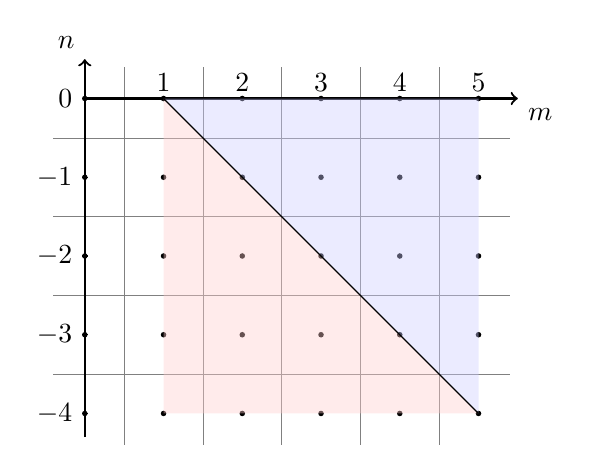
\begin{tikzpicture}
    \draw[step=1cm,gray,very thin, xshift=0.5cm, yshift=-0.5cm] (-0.9,0.9) grid (4.9,-3.9);
    \draw[thick,->] (0,0) -- (5.5,0) node[anchor=north west] {\( m \)};
    \draw[thick,->] (0,-4.3) -- (0,0.5) node[anchor=south east] {\( n \)};
    \foreach \x in {1,2,3,4,5}
    \draw (\x cm,1pt) -- (\x cm,-1pt) node[anchor=south] {$\x$};
    \foreach \y in {0, -1,-2,-3,-4}
    \draw (1pt,\y cm) -- (-1pt,\y cm) node[anchor=east] {$\y$};

    \foreach\x in {0,...,5} {
      \foreach \y in {0,-1,-2,-3,-4} {
        \fill (\x, \y) circle[radius=1pt];
      }
    }
    % \fill[blue!20, opacity=0.4] (-0.5, 0) -- (4, -4.5) -- (-0.5, -4.5) -- (-0.5, 0);
    % \fill[red!20, opacity=0.4] (0, -0.5) -- (4.5, -5) -- (4.5, -0.5) -- (0, -0.5);
    \fill[blue!20, opacity=0.4] (1, 0) -- (5, -4) -- (5, 0) -- (1, 0);
    \fill[red!20, opacity=0.4] (1,0) -- (5, -4) -- (1, -4) -- (1,-1);
    \draw (1, 0) -- (5, -4);
  \end{tikzpicture}
  \caption{The region of \( (m,n) \) to sum over for a Type-I perpendicularly tilted cone.
    The black line represents the combinations that give a finite contribution also in the untilted case.
    As the cone is tilted, this sharp line ``diffuse'' into the red and blue regions as well.
    Note that, as \( \Xi_1 \) defined only for \( M>0\), the region with \( m=0 \) gives no contribution.}
  \label{fig:nmregion}
\end{figure}

\begin{figure}[ht]
  \centering
  \pgfplotsset{
    % colormap={X}{ gray(0cm)=(1); gray(1cm)=(0);},
    % colormap={mycool}{ rgb255(0)=(255,0,255); rgb255(8)=(0,128,255); rgb255(10)=(255,255,255);},
    colormap={temp}{rgb255=(36,0,217) rgb255=(25,29,247) rgb255=(41,87,255)
      rgb255=(61,135,255) rgb255=(87,176,255) rgb255=(117,211,255) rgb255=(153,235,255)
      rgb255=(255,255,255)
      rgb255=(255,214,153) rgb255=(255,172,117) rgb255=(255,120,87) rgb255=(255,61,61)
      rgb255=(247,40,54) rgb255=(217,22,48) rgb255=(166,0,33)},
    % colormap={mycool}{ rgb255(-1)=(255,0,255); rgb255(-0.1)=(255,0,255); rgb255(0)=(255,255,255); rgb255(1)=(0,128,255)},
    % colormap={violet}{rgb255=(25,25,122) color=(white) rgb255=(238,140,238)},
    point meta min=-0.1,
    point meta max=0.1,
    xlabel=\( m \),
    ylabel=\( n \),
  }
  \newcounter{plotnum}
  \subcaptionbox{Inversion symmetric case.\label{fig:contribs:P}}{
    \begin{tikzpicture}
      \begin{groupplot}[
        width=0.4\textwidth,
        axis equal,
        xmin=-6, xmax=6,
        ymin=-6, ymax=6,
        % title={\( t_x= \title \)},
        title style={ at={(0.7, 0.7)} },
        group style={
          group size=2 by 2,
          group name=contribs,
          x descriptions at=edge bottom,
          y descriptions at=edge left,
          horizontal sep=8pt,
          vertical sep=8pt,
        },
        ]
        \pgfplotsforeachungrouped \datafile/\title in {
          contribTilttx0.PbrokenFalse.csv/0,
          contribTilttx0.125PbrokenFalse.csv/0.16,
          contribTilttx0.25PbrokenFalse.csv/0.25,
          contribTilttx0.5PbrokenFalse.csv/0.5
        }{
          \edef\tmp{
            \noexpand\ifthenelse{\theplotnum=1}{
              \noexpand\nextgroupplot[title={$t_x = \title$}, colorbar right,
              every colorbar/.append style={height=
                2*\noexpand\pgfkeysvalueof{/pgfplots/parent axis height}+8pt},
              colorbar to name={mycolorbar}
              ]
              % See  https://tex.stackexchange.com/questions/126177/common-colorbar-for-groupplot
            }{
              \noexpand\nextgroupplot[title={$t_x = \title$}]
            }
            % \noexpand\nextgroupplot[title={$t_x = \title$}, colorbar, colorbar horizontal, colorbar to name={mycolorbar}]
            \noexpand\addplot [
            matrix plot*,
            mesh/cols=13,
            point meta=explicit,
            ] table[x=m, y=n, meta=Contrib, col sep=comma] {data/\datafile};
          }
          \tmp
          \stepcounter{plotnum}
        }
      \end{groupplot}
      %% Shfit half vertical sep
      \node[anchor=west, yshift=4pt] at (contribs c2r2.north east) {\ref{mycolorbar}};
    \end{tikzpicture}
  } %% Subcaptionbox end

  \subcaptionbox{Inversion symmetry broken case.\label{fig:contribs:Pbroken}}{
    \begin{tikzpicture}
      \begin{groupplot}[
        width=0.4\textwidth,
        axis equal,
        xmin=-6, xmax=6,
        ymin=-6, ymax=6,
        % title={\( t_x= \title \)},
        title style={ at={(0.7, 0.7)} },
        group style={
          group size=2 by 2,
          group name=contribs,
          x descriptions at=edge bottom,
          y descriptions at=edge left,
          horizontal sep=8pt,
          vertical sep=8pt,
        },
        ]
        \setcounter{plotnum}{0}
        \pgfplotsforeachungrouped \datafile/\title in {
          contribTilttx0.PbrokenTrue.csv/0,
          contribTilttx0.125PbrokenTrue.csv/0.16,
          contribTilttx0.25PbrokenTrue.csv/0.25,
          contribTilttx0.5PbrokenTrue.csv/0.5
        }{
          \edef\tmp{
            \noexpand\ifthenelse{\theplotnum=1}{
              \noexpand\nextgroupplot[title={$t_x = \title$}, colorbar right,
              every colorbar/.append style={height=
                2*\noexpand\pgfkeysvalueof{/pgfplots/parent axis height}+8pt},
              colorbar to name={mycolorbar}
              ]
              % See  https://tex.stackexchange.com/questions/126177/common-colorbar-for-groupplot
              %
            }{
              \noexpand\nextgroupplot[title={$t_x = \title$}]
            }

            % \noexpand\nextgroupplot[title={$t_x = \title$}, colorbar, colorbar horizontal, colorbar to name={mycolorbar}]
            \noexpand\addplot [
            matrix plot*,
            mesh/cols=13,
            point meta=explicit,
            ] table[x=m, y=n, meta=Contrib, col sep=comma] {data/\datafile};
          }
          \tmp

          \ifthenelse{\theplotnum=0}{
            \draw[dotted, gray] (axis cs:-1.5,-1.5) rectangle (axis cs:1.5,1.5) node[pos=0, pin={[pin edge={solid}]-180:\( \gamma_0 \)}] {};
            \draw[dotted, gray] (axis cs:-2.5,-2.5) rectangle (axis cs:2.5,2.5) node[pos=0, pin={[pin edge={solid}]-110:\( \gamma_1 \)}] {};
          }{}
          \stepcounter{plotnum}
        }
      \end{groupplot}
      %% Shfit half vertical sep
      \node[anchor=west, yshift=4pt] at (contribs c2r2.north east) {\ref{mycolorbar}};
    \end{tikzpicture}
  }
  \caption{Contributions to \( \gamma_N \) from \( m\to n \) transitions for different values of \( t_x \).
    TODO: Update caption
    \label{fig:contribs}
    }
\end{figure}

\subsection{Tilt parallell to the magnetic field}
We consider here a tilt parallel to the magnetic field, \( \vec{t} \parallel \vec{B} \). We will consider only the canonical part of the energy-momentum tensor, and not the full symmetrized form, as described \citeauthor{vanderwurffMagnetovorticalThermoelectricTransport2019} \cite{vanderwurffMagnetovorticalThermoelectricTransport2019}.
\begin{equation}
  \label{eq:103}
  T^{\mu 0} = \frac{i}{2}
  [
  \partial_j \bar{\psi} \Gamma ^j \gamma ^0 \Gamma ^{\mu } \psi - \bar{\psi} \Gamma ^{\mu } \gamma ^0 \Gamma ^j \partial _j \psi
  ],
\end{equation}
where \( \Gamma ^{\mu } = \gamma ^{\mu } + \gamma ^0 t^{\mu } \) with \( t^{\mu } = (0, \vec{t}) \) when inversion symmetry is broken and \( \Gamma ^{\mu }= \gamma ^{\mu } = \gamma ^0 \gamma ^5 t^{\mu } \) in the inversion symmetric case.

We have, with \( \vec{t}^{\chi } = \vec{t} \) in the inversion symmetric case, and \( \vec{t}^{\chi } = \vec{t} \) in the symmetry broken case.
The expression is exactly the same as for the untilted case, only with different energies.
The dimensionless quantities are
\begin{equation}
  \label{eq:104}
  \epsilon_{\kappa m s} =
  \begin{cases}
    t_z^{\chi } \kappa + \sign{m} \sqrt{M + \kappa ^2} & m \neq 0\\
    (t_z^{\chi } - s) \kappa & m = 0
  \end{cases}.
\end{equation}
The normalization factor \( \alpha _{\vec{k} m s} \) is, expressed in dimensionless quantities,
\begin{equation}
  \label{eq:105}
  \alpha _{\kappa m s} =
  -\sqrt{\frac{M}{(\epsilon_{\kappa  m s} - t_{z}^{\chi })s - \kappa }}.
\end{equation}
The integrand is
\begin{equation}
  \label{eq:106}
  \sum\limits_{mn}^{}
  (\epsilon_{\kappa m s} + \epsilon_{\kappa n s}) (\alpha_{\kappa m s}^2 \delta_{M, N+1} - \alpha_{\kappa n s}^2 \delta _{N, M+1}).
\end{equation}
\todo{Make sure to use the same conventions (choice of quadrants etc) as in untilted case}
As described above, the contributions from the \( \alpha _{\kappa n s}^2  \) and \( \alpha _{\kappa m s}^2 \) terms are identical, and we may simply take
\begin{equation}
  \label{eq:107}
  \sum\limits_{\underset{N=M-1}{mn}}^{}
  (\epsilon_{\kappa m s} + \epsilon_{\kappa n s}) \alpha_{\kappa m s}^2.
\end{equation}
As was the case in the untilted system, the integrand is also now invariant under \( (m, n, \kappa_z) \mapsto (-m, -n, -\kappa_z) \), and we may consider only half the \( m,n \) plane, adding a degeneracy factor 2.

Even though the treatment above for a general tilt is valid for parallel tilt, the response can be found more directly from the untilted case.
For \( \vec{t} = t_z \hat{z} \), the energy momentum tensor \( T^{0y} \), charge current \( J^x \), and wave functions \( \phi(\vec{r}) \) are all independent of \( t_z \), and the only difference compared to the untilted system is a change in the energies of the Landau levels.
We may thus immediately use the result from the untilted case
\begin{equation}
  \label{eq:129}
  \lim_{\omega \to 0} \lim_{\vec{q} \to 0} \chi^{xy} =
  - \frac{e^2 v_F B}{4(2\pi)^2}
  \sum\limits_{mn} \int \mathrm{d} \kappa_z
  \xi(\kappa_z)
  (\epsilon_{\kappa_z m s} + \epsilon_{\kappa_z n s})
  (\alpha_{\kappa_z m s}^2 \delta_{M-1, N} - \alpha_{\kappa_z n s}^2 \delta_{N-1, M}).
\end{equation}
In the untilted case we made several simplifications to this expression, especially with regards to limiting the summation domain.
We will here consider which of those simplifications apply also in the case of tilt \( t_z \).

Under the transformation \( (m,n,\kappa_z) \mapsto (-m, -n , -\kappa_z) \), \( \xi(\kappa_z), \epsilon_{\kappa_z m s}, \alpha_{\kappa_z m s} \) are all still odd, and so the integrand is invariant under such a transformation.
As the integral is over all \( \kappa_z \), we may therefore consider only half the \( m,n \) plane, as was the case in the untilted case.
However, in the untilted case the sum was in fact restricted to only one quadrant, as at \( T\to 0 \) the transitions must be between states with energy of opposite sign.
In the case of Type-II systems, this requirement does not restrict the sum to one quadrant.
It is thus convenient to consider Type-I and Type-II separately.

In the untitled system, the contributions from the two chiralities where the same, as \( \kappa_z \) and \( s \) always appeared in conjunction, \( \kappa_z s \).
In the case of \( t_z \) tilt, this is not the case.
The tilt parameter enters the expression only through \( \epsilon_{\kappa_z m s} = \epsilon_{\kappa_z m s}^0 + \kappa_z t^s_z \).
The proof for the response from the two chiralities being the same in the untilted case was that \( s \) and \( \kappa_z \) appeared only through the product \( s \kappa_z \), and so the expression was invariant under \( (s, \kappa_z) \mapsto (-s, -\kappa_z) \).
As our integration spans all \( \kappa_z \), the total response is invariant under \( s \to -s \).
In the inversion symmetric case, \( t^s_z = s t_z \), this argument still holds.
In the case of broken inversion symmetry, however, where \( t^s_z = t_z \), the argument fails.
A similar argument may, however, be made for the transformation \( (s, \kappa_z, t_z) \mapsto (-s, -\kappa_z, -t_z) \), for which the (inversion broken) system is invariant.
The response of a cone with chirality \( s = -1 \) is thus equal the response with \( s = +1 \) and \( t_z \to -t_z \).
We therefore compute all responses for \( s=+1 \);
for symmetric systems the response is equal for \( s=-1 \), while for broken inversion symmetry, the response is given at \( t_z \to -t_z \).

\subsubsection{Type-I}
In Type-I systems, the selection rules from the step functions are independent of \( t_z \), and the only difference from the untilted case is the term \( \epsilon_{\kappa_z m s} + \epsilon_{\kappa_z n s} = \epsilon^0_{\kappa_z m s} + \epsilon^0_{\kappa_z n s} + 2 \kappa_z t^s_z \).
We compute therefore only the term that differ, for \( s=+1 \).
The integral
\begin{equation}
  \label{eq:97}
  \frac{\gamma_{\text{div}, N}}{2} = \int \mathrm{d}\kappa_z \xi(\kappa_z) \kappa_z t_z \alpha_{\kappa_z m s}^2
\end{equation}
diverges.
Introduce the momentum cutoff \( \Lambda \), in which case the integral can be solved analytically, with the result
\begin{multline}
  \frac{t_z}{4}
  \Bigg\{
    \Lambda\left(\sqrt{1 + \Lambda^2 + m} - \sqrt{\Lambda^2 + m}  \right)\\
    + m \tanh^{-1}\left[\frac{\Lambda}{\sqrt{\Lambda^2 + m} } \right]
    - (m+1) \tanh^{-1}\left[\frac{\Lambda}{\sqrt{1 + \Lambda^2 + m }}\right]
    \Bigg\},
    \label{eq:98}
\end{multline}
where we used the selection rule of the sum \( N=M+1 \) and \( m>0, n<0 \).
This contribution is shown in figure \ref{fig:divergent-factor}.
\todo{is it ok to write 'the contribution \eqref{eq:98}', or must it always be 'the contribution Eq. \eqref{eq:98}'?}
The contribution \eqref{eq:98} is odd in \( t_z \), and so for systems with broken inversion symmetry, the total contribution from two cones cancel.


\subsubsection{Type-II}
\todo{Recheck the order and specify clearly if we consider Type-I or Type-II for the different arguments}
\todo{There should be some argument along the lines of the result being the same for s -> -s and tz -> -tz, so we may consider s=1, tz>0 for defiteness (if that is indeed the case)}

% % Computing this in PGF was no good.
% % Import from a file instead
% \begin{tikzpicture}
%   \pgfkeys{/pgf/declare function={arctanh(\x)=0.5*(ln((1+\x)/(1-\x)));}}
%   \pgfkeys{/pgf/declare function={divLim(\x,\z,\m)=-0.25 * \z * (
%       \x (sqrt(1 + \x^2 + \m) - sqrt(\x^2 + \m)) +
%       \m * arctanh(\x/sqrt(\x^2 + \m)) - (\m+1)*arctanh(\x/sqrt(1 + \x^2 + \m))
%       );}}
%   \begin{axis}[
%     domain=0:100,
%     samples=50,
%     ]
%     \addplot[mark=none] {divLim(x, 0.1,1)};
%   \end{axis}
% \end{tikzpicture}

\begin{figure}[hp]
  \centering
  \tikzsetnextfilename{divergentContribCutoff}
  \begin{tikzpicture}
    \begin{axis}[
      xlabel=\( \Lambda \),
      ylabel=Contribution,
      legend pos=south east,
      ]
      \foreach \i in {1,...,5} {
        \addplot+[mark=none] table[x index=0, y index=\i, col sep=comma] {data/divergentFactor.csv};
        \addlegendentryexpanded{\( m = \i \)};
      }
    \end{axis}
  \end{tikzpicture}
  \caption{The divergent factor \( \gamma_{\text{div}, N} / t_{z} \) for the first Landau levels, as a function of the momentum cutoff \( \Lambda \).
    TODO: fix m to be m-1. Alternatively use N}
  \label{fig:divergent-factor}
\end{figure}
For Type-I semimetals, the sign of energy state \( m \neq 0 \) is given by the sign of \( m \) itself.
For \( m = 0 \) the sign of the energy is given by \( -s \sign{\kappa } \).
Due to this, the sum is restricted to \( n=M+1, m=-M \) and \( n=-M-1, m=M \).
In the case of Type-II, however, the situation is not so simple.
The energy bands cross the Fermi surface, and we must also include in our sum overlap between states of the same sign, i.e. \( n=M+1, m=M \) and \( n=-M-1, m=-M \), which is non-zero for certain intervals of \( \kappa  \).
See figure \ref{fig:llevelstilt}.

% Furthermore, the expression is no longer invariant under \( (s, \kappa_z) \mapsto (-s, -\kappa_z) \).
% For inversion symmetric systems, \( \vec{t^s} = s \vec{t} \), the symmetry is still conserved, however, for broken inversion symmetry, the extra term in the energies, \( t^s_z \kappa_z \) breaks the symmetry between the chiralitites.
% As the energies change between the chiralities, so does the step function, giving other selection rules.
% For inversion symmetric systems, we may thus simply choose a value of \( s \), for example \( s=1 \), and compute all results for that value.
% For broken inversion symmetry, however, the results must be computed separately for the two chiralities.
% \todo{Or maybe it is easier to do all calculations with \( t_x^s \) (and its sign) in focus, and then later apply inversion (broken) symmetry?}

In order to find explicitly the limits of integration for the Type-II case, we must find the roots of the energy levels.
The zeroth Landau level always has only one root, which is in the origin.
For the higher order Landau levels, we solve
\begin{equation}
  \label{eq:93}
  \epsilon_{\kappa_z m s } = t_z^s \kappa_z + \sign(m) \sqrt{M + \kappa_{z} ^2} = 0,
\end{equation}
whose solution is
\[
\kappa_z^2 = \frac{M}{t_{z}^2 - 1}.
\]
The actual roots of the energies are
\begin{equation}
  \label{eq:94}
  \kappa_z = -\sign(m t^s_x) \sqrt{\frac{M}{t_{z}^2 - 1}}.
\end{equation}
The integration limit for the \( 0 \to 1 \) transition is thus, for \( t_z^s > 1 \), \( [-\sqrt{t_z^2 - 1 }^{-1}, 0] \).
The \( 1\to 2 \) transition is \( [-\sqrt{2} /\sqrt{t_z^2 - 1}, -\sqrt{t_z^2 - 1 }^{-1}] \), and so forth.

The \( 0\to 1 \) transitions where computed analytically, and found to be
\begin{equation}
  \label{eq:117}
  \frac{\sign(t_z)}{2}
  \left(
  |t_z| \sinh^{-1}\left(\frac{1}{\sqrt{t_{z}^2-1} }\right) -1
\right  ).
\end{equation}
For a general \( -N \to N+1, \; N>0 \) transition, the contribution was found to be the very lengthy expression
\todo{Must also do \( t_z < -1 \)}
\todo{Be careful with tz < -1. This does not only change sing of tz, but also the integration limits}
\begin{multline}
  \label{eq:132}
  \frac{(n-1) n }{8
   ((n-1) n)^{3/2} (t_z^2-1)}
 \Bigg[
   n t_z\\
   \left(F_1\left(1;\frac{1}{2},\frac{1}{2};2;\frac{1}{1-t_z^2},-\frac{n}{(n-1)
         (t_z^2-1)}\right)
     -F_1\left(1;\frac{1}{2},\frac{1}{2};2;\frac{1-n}{n
   (t_z^2-1)},\frac{1}{1-t_z^2}\right)\right)\\
%%
+t_z
   F_1\left(1;\frac{1}{2},\frac{1}{2};2;\frac{1-n}{n
       (t_z^2-1)},\frac{1}{1-t_z^2}\right)
   +n^2 (4-4 t_z^2)
   \sqrt{(n-1) ((n-1) t_z^2+1)}\\
%%
   -4 \sqrt{(n-1) n} n^2 (t_z^2-1)
   \log \left(\frac{\sqrt{\frac{n-1}{n}} \left(\sqrt{1-n t_z^2}+\sqrt{1-n}\right)}{\sqrt{-n
         t_z^2+t_z^2-1}+\sqrt{-n}}\right)\\
   %%
   -n (2-2 t_z) \sqrt{(1-n) \left(-((n-1)
   t_z^2)-1\right)}+2 n (t_z-1) t_z \sqrt{(n-1) \left((n-1)
 t_z^2+1\right)}\\
%%
+(1-n) n \left(4-4 t_z^2\right) \sqrt{-n \left(1-n
    t_z^2\right)}+2 (1-n) \left(t_z^2-1\right) \sqrt{-n \left(1-n t_z^2\right)}\\
%%
-2
\sqrt{(n-1) n} (t_z^2-1) \Bigg[
-t_z \log \left(-\left((t_z-1)
         \sqrt{\frac{1-n}{t_z^2-1}}\right)\right)\\
     %%
     -t_z \log \left(\frac{\sqrt{-n
   t_z^2+t_z^2-1}+\sqrt{-n}}{\sqrt{t_z^2-1}}\right)+t_z \log
(1-n)-1
\Bigg]\\
%%
+2 \sqrt{(n-1) n} n \left(-t_z^3-2 t_z^2+t_z+2\right) \log
   \left(\frac{\sqrt{\frac{n}{n-1}} \left(\sqrt{-n
           t_z^2+t_z^2-1}+\sqrt{-n}\right)}{\sqrt{1-n t_z^2}+\sqrt{1-n}}\right)\Bigg]
, \text{ for  } t_z<-1
\end{multline}
and
\begin{multline}
  \label{eq:133}
  \frac{1}{8
   \sqrt{(n-1) n} \left(t_z^2-1\right)}
 \Bigg\{
 n t_z \Bigg(\\
   %%
   F_1\left(1;\frac{1}{2},\frac{1}{2};2;\frac{1-n}{n
       \left(t_z^2-1\right)},\frac{1}{1-t_z^2}\right)\\
   %%
   -F_1\left(1;\frac{1}{2},\frac{1}{2};2;
     \frac{1}{1-t_z^2},-\frac{n}{(n-1) \left(t_z^2-1\right)}\right)
 \Bigg)\\
 %%
 -t_z
   F_1\left(1;\frac{1}{2},\frac{1}{2};2;\frac{1-n}{n
       \left(t_z^2-1\right)},\frac{1}{1-t_z^2}\right)\\
   %%
   +n^2 (4-4 t_z^2)
   \sqrt{(n-1) \left((n-1) t_z^2+1\right)}\\
   %%
   +4 n^2 (t_z^2-1) \sqrt{n \left(n
       t_z^2-1\right)}\\
   %%
   -4 \sqrt{(n-1) n} n^2 \left(t_z^2-1\right) \log
   \left(\frac{-\sqrt{(n-1) \left(n t_z^2-1\right)}+n-1}{n \sqrt{\frac{(n-1)
           t_z^2+1}{n}}+n}\right)\\
   %%
   +2 n \left(t_z^2-1\right) \sqrt{(n-1) \left((n-1)
       t_z^2+1\right)}\\
   %%
   +n \left(6-6 t_z^2\right) \sqrt{n \left(n t_z^2-1\right)}\\
   %%
   +2
   \left(t_z^2-1\right) \sqrt{n \left(n t_z^2-1\right)}\\
   %%
   -2 \sqrt{(n-1) n}
   \left(t_z^2-1\right) \Bigg(-t_z \log \left((t_z+1)
     \sqrt{\frac{1-n}{t_z^2-1}}\right)\\
   %%
   -t_z \log \left(\frac{\sqrt{-n
         t_z^2+t_z^2-1}+\sqrt{-n}}{\sqrt{t_z^2-1}}\right)\\
   %%
   +t_z \log
   (1-n)+1
   \Bigg)\\
   %%
   +2 \sqrt{(n-1) n} n \left(-t_z^3-2 t_z^2+t_z+2\right) \log
   \left(\frac{\sqrt{\frac{n}{n-1}} \left(\sqrt{-n
           t_z^2+t_z^2-1}+\sqrt{-n}\right)}{\sqrt{1-n t_z^2}+\sqrt{1-n}}\right)
   \Bigg\}, \text{ for } t_z > 1.
\end{multline}

% \begin{multline}
%   \frac{1}{8 \sqrt{(n-1) n} \left(t_z^2-1\right)}
%   \Bigg\{
%     -n t_z F_1\left(1;\frac{1}{2},\frac{1}{2};2;\frac{1}{1-t_z^2},-\frac{n}{(n-1)
%         \left(t_z^2-1\right)}\right)\\
%     %%
%     +(n-1) t_z
%     F_1\left(1;\frac{1}{2},\frac{1}{2};2;\frac{1-n}{n
%         \left(t_z^2-1\right)},\frac{1}{1-t_z^2}\right)\\
%     %%
%     +\left(t_z^2-1\right)
%     \Bigg[
%       \sqrt{(n-1) n} \Big\{-4 n^2 \log \left(\frac{-\sqrt{(n-1) \left(n
%                 t_z^2-1\right)}+n-1}{n \sqrt{\frac{(n-1) t_z^2+1}{n}}+n}\right)\\
%         %%
%         +n (t_z+2)
%         \left(2 \log \left(\frac{\sqrt{1-n t_z^2}+\sqrt{1-n}}{\sqrt{-n
%                 t_z^2+t_z^2-1}+\sqrt{-n}}\right)+\log (n-1)-\log (n)\right)\\
%         %%
%         -2 t_z \log
%         \left(\frac{n (-t_z)+n+t_z-1}{\sqrt{(n-1)^2 t_z^2+n-1}+\sqrt{(n-1)
%               n}}\right)\Big\}\\
%         %%
%       +2 \Big(n \left(-2 n \sqrt{(n-1)^2 t_z^2+n-1}+2 n \sqrt{n \left(n
%               t_z^2-1\right)}+\sqrt{(n-1)^2 t_z^2+n-1}-3 \sqrt{n \left(n
%               t_z^2-1\right)}\right)\\
%         %%
%         +\sqrt{n \left(n t_z^2-1\right)}-\sqrt{(n-1)
%           n}\Big)
%       \Bigg]
%     \Bigg\}.
% \end{multline}
where \( F_1 \) is the Appell hypergeometric function of two variables.

As described above, for broken inversion symmetry, the result of the chirality \( s=-1 \) is that of \( s=+1 \) at \( t_z \to -t_z \).
The total contribution will therefore be the sum of the contribution for \( t_z > 1 \) an d\( t_z < -1 \), which is
\begin{multline}
  \label{eq:134}
  \frac{1}{4 \sqrt{(n-1) n} \left(t_z^2-1\right)}
  \Bigg\{
  | t_z|  \Bigg((n-1) F_1\left(1;\frac{1}{2},\frac{1}{2};2;\frac{1-n}{n
        \left(t_z^2-1\right)},\frac{1}{1-t_z^2}\right)\\
    %%
    -n
    F_1\left(1;\frac{1}{2},\frac{1}{2};2;\frac{1}{1-t_z^2},-\frac{n}{(n-1)
        \left(t_z^2-1\right)}\right)
  \Bigg)\\
  %%
  +2 \left(t_z^2-1\right) \Bigg(-2 n^2 \sqrt{(n-1)
      \left((n-1) t_z^2+1\right)}+2 n^2 \sqrt{n \left(n t_z^2-1\right)}\\
    %%
    -\sqrt{(n-1) n} n^2
    \log \left(\frac{\sqrt{\frac{n-1}{n}} \left(\sqrt{1-n t_z^2}+\sqrt{1-n}\right)}{\sqrt{-n
          t_z^2+t_z^2-1}+\sqrt{-n}}\right)\\
    %%
    -\sqrt{(n-1) n} n^2 \log \left(\frac{-\sqrt{(n-1)
          \left(n t_z^2-1\right)}+n-1}{n \sqrt{\frac{(n-1) t_z^2+1}{n}}+n}\right)\\
    %%
    +n
    \sqrt{(n-1) \left((n-1) t_z^2+1\right)}-3 n \sqrt{n \left(n t_z^2-1\right)}+\sqrt{n
      \left(n t_z^2-1\right)}\\
    %%
    -2 \sqrt{(n-1) n} n \log \left(\frac{\sqrt{\frac{n}{n-1}}
        \left(\sqrt{-n t_z^2+t_z^2-1}+\sqrt{-n}\right)}{\sqrt{1-n
          t_z^2}+\sqrt{1-n}}\right)\Bigg)
  \Bigg\}
\end{multline}


% \fbox{
%   The unsimplified \( n\to m, n<0, m>0 \) transition
%   $$
%   \frac{1}{4} m \left(\frac{-\frac{\text{tz}
%    F_1\left(1;\frac{1}{2},\frac{1}{2};2;\frac{1}{1-\text{tz}^2},\frac{m}{n
%    \left(\text{tz}^2-1\right)}\right)}{\text{tz}^2-1}-\frac{m \sqrt{-m n} (n (\text{tz}-2)+m
%    \text{tz}) \log (m)+n \sqrt{-m n} (n \text{tz}+m (\text{tz}+2)) \log (-n)-2 \left(-n m^2+n
%    \text{tz} m^2-\sqrt{-m n} m^2+\sqrt{-m n \left(-n \text{tz}^2+m+n\right)} m^{3/2}-n^2 m-n^2
%    \text{tz} m+\sqrt{-m n} (n (\text{tz}-2)+m \text{tz}) \log \left((\text{tz}+1)
%    \sqrt{\frac{m}{\text{tz}^2-1}}\right) m-n \sqrt{-n \left(-n \text{tz}^2+m+n\right)} m+(-m
%    n)^{3/2}+n \sqrt{-m n} (n \text{tz}+m (\text{tz}+2)) \log \left(\frac{\sqrt{m}+\sqrt{-n
%    \text{tz}^2+m+n}}{\sqrt{\text{tz}^2-1}}\right)\right)}{m (m+n)^2}}{2 \sqrt{-m n}}+\frac{\sqrt{-n}
%    \text{tz} F_1\left(1;\frac{1}{2},\frac{1}{2};2;\frac{n}{m
%    \left(\text{tz}^2-1\right)},\frac{1}{1-\text{tz}^2}\right) (m+n)^2+\sqrt{m} \left(-m (n
%    (\text{tz}-2)+m \text{tz}) \left(\text{tz}^2-1\right) \log (m)-n \left(\text{tz}^2-1\right) (n
%    \text{tz}+m (\text{tz}+2)) \log (-n)+2 \left(-\frac{n^2 \text{tz}^4}{\text{tz}^2-1}-\frac{m n
%    \text{tz}^4}{\text{tz}^2-1}+m \sqrt{-m n} \text{tz}^3-n \sqrt{-m n} \text{tz}^3-\frac{m \sqrt{-n
%    \left(m \text{tz}^2-m-n\right)} \text{tz}^3}{\text{tz}^2-1}-\frac{n \sqrt{-n \left(m
%    \text{tz}^2-m-n\right)} \text{tz}^3}{\text{tz}^2-1}-\frac{n^2 \text{tz}^3}{\text{tz}^2-1}+\frac{m
%    n \text{tz}^3}{\text{tz}^2-1}-m \sqrt{-m n} \text{tz}^2-n \sqrt{-m n} \text{tz}^2-m \sqrt{n
%    \left(-m \text{tz}^2+m+n\right)} \text{tz}^2+n \sqrt{n \left(-m \text{tz}^2+m+n\right)}
%    \text{tz}^2+\frac{m \sqrt{-n \left(m \text{tz}^2-m-n\right)} \text{tz}^2}{\text{tz}^2-1}-\frac{n
%    \sqrt{-n \left(m \text{tz}^2-m-n\right)} \text{tz}^2}{\text{tz}^2-1}+\frac{n^2
%    \text{tz}^2}{\text{tz}^2-1}+\frac{m n \text{tz}^2}{\text{tz}^2-1}+n^2 \text{tz}-m n \text{tz}-m
%    \sqrt{-m n} \text{tz}+n \sqrt{-m n} \text{tz}+m \sqrt{n \left(-m \text{tz}^2+m+n\right)}
%    \text{tz}+n \sqrt{n \left(-m \text{tz}^2+m+n\right)} \text{tz}+\frac{m \sqrt{-n \left(m
%    \text{tz}^2-m-n\right)} \text{tz}}{\text{tz}^2-1}+\frac{n \sqrt{-n \left(m
%    \text{tz}^2-m-n\right)} \text{tz}}{\text{tz}^2-1}+\frac{n^2 \text{tz}}{\text{tz}^2-1}-\frac{m n
%    \text{tz}}{\text{tz}^2-1}+n^2+m n+n \left(\text{tz}^2-1\right) (n \text{tz}+m (\text{tz}+2)) \log
%    \left((\text{tz}+1) \sqrt{-\frac{n}{\text{tz}^2-1}}\right)+m (n (\text{tz}-2)+m \text{tz})
%    \left(\text{tz}^2-1\right) \log
%    \left(\sqrt{-\frac{n}{\text{tz}^2-1}}+\sqrt{m+\frac{n}{1-\text{tz}^2}}\right)+m \sqrt{-m n}+n
%    \sqrt{-m n}-\frac{m \sqrt{-n \left(m \text{tz}^2-m-n\right)}}{\text{tz}^2-1}+\frac{n \sqrt{-n
%    \left(m \text{tz}^2-m-n\right)}}{\text{tz}^2-1}\right)\right)}{2 m^{3/2} (m+n)^2
%    \left(\text{tz}^2-1\right)}\right)
% $$
% } %% fbox

% \fbox{
%   The simplified transition
%   $$
% \frac{-m^{3/2} \text{tz} (m+n)^2
%    F_1\left(1;\frac{1}{2},\frac{1}{2};2;\frac{1}{1-\text{tz}^2},\frac{m}{n
%    \left(\text{tz}^2-1\right)}\right)-\sqrt{m} n \text{tz} (m+n)^2
%    F_1\left(1;\frac{1}{2},\frac{1}{2};2;\frac{n}{m
%    \left(\text{tz}^2-1\right)},\frac{1}{1-\text{tz}^2}\right)+2 \left(\text{tz}^2-1\right)
%    \left(\sqrt{-m^5 n \left(m-n \text{tz}^2+n\right)}-n \sqrt{-m^3 n \left(m-n
%    \text{tz}^2+n\right)}+m^3 \sqrt{-n} \text{tz} \log \left((\text{tz}+1)
%    \sqrt{\frac{m}{\text{tz}^2-1}}\right)+m^3 \sqrt{-n} \text{tz} \log
%    \left(\sqrt{m-\frac{n}{\text{tz}^2-1}}+\sqrt{\frac{n}{1-\text{tz}^2}}\right)-m^3 \sqrt{-n}+m^2 n
%    \sqrt{m \left(\text{tz}^2-1\right)-n}+2 m^2 \sqrt{-n} n \log \left((\text{tz}+1)
%    \sqrt{\frac{n}{1-\text{tz}^2}}\right)+m^2 \sqrt{-n} n \text{tz} \log \left((\text{tz}+1)
%    \sqrt{\frac{n}{1-\text{tz}^2}}\right)+2 m^2 (-n)^{3/2} \log \left((\text{tz}+1)
%    \sqrt{\frac{m}{\text{tz}^2-1}}\right)+m^2 \sqrt{-n} n \text{tz} \log \left((\text{tz}+1)
%    \sqrt{\frac{m}{\text{tz}^2-1}}\right)+2 m^2 \sqrt{-n} n \log \left(\frac{\sqrt{m-n
%    \text{tz}^2+n}+\sqrt{m}}{\sqrt{\text{tz}^2-1}}\right)+m^2 \sqrt{-n} n \text{tz} \log
%    \left(\frac{\sqrt{m-n \text{tz}^2+n}+\sqrt{m}}{\sqrt{\text{tz}^2-1}}\right)+2 m^2 (-n)^{3/2} \log
%    \left(\sqrt{m-\frac{n}{\text{tz}^2-1}}+\sqrt{\frac{n}{1-\text{tz}^2}}\right)+m^2 \sqrt{-n} n
%    \text{tz} \log \left(\sqrt{m-\frac{n}{\text{tz}^2-1}}+\sqrt{\frac{n}{1-\text{tz}^2}}\right)-m^2
%    \sqrt{-n} \log (m) (m \text{tz}+n (\text{tz}-2))+2 m^2 (-n)^{3/2}-m n^2 \sqrt{m
%    \left(\text{tz}^2-1\right)-n}+m (-n)^{5/2} \text{tz} \log \left((\text{tz}+1)
%    \sqrt{\frac{n}{1-\text{tz}^2}}\right)+m (-n)^{5/2} \text{tz} \log \left(\frac{\sqrt{m-n
%    \text{tz}^2+n}+\sqrt{m}}{\sqrt{\text{tz}^2-1}}\right)+m (-n)^{3/2} \log (-n) (m (\text{tz}+2)+n
%    \text{tz})+m (-n)^{3/2} n\right)}{8 m \sqrt{-n} \left(\text{tz}^2-1\right) (m+n)^2}
% $$
% } %% fbox
\section{Results}
We will here consider parallel and perpendicular tilt separately.
\todo{Make sure the argumentation and computations are valid also for \( t_z < 0 \)}

\subsection{Perpendicular tilt}
In the case of a tilt perpendicular to the magnetic field, we are, as previously explained, restricted to Type-I materials, as the Landau level description breaks down for Type-II perpendicular tilt.
Importantly, this does not generally mean that the effect is not present for Type-II systems, but simply that the Linear model Landau level description is not a good basis for the system.
The collapse of the Landau levels caused \textcite{soluyanovTypeIIWeylSemimetals2015} to errenously predict the collapse of the chiral anomaly in their now famous paper first describing Type-II Weyl semimetals.

As explained in section \ref{sec:perptiltsum}, the \( m,n \) summation is restricted to the fourth quadrant in the \( m,n \) plane.
In the case of no tilt, only contributions from \( M = N + 1 \) were non-zero;
we named the contribution from the \( 0\to 1 \) transition \( \gamma_0 \), the \( -1\to 2 \) transition \( \gamma_1 \) and so fourth.
Here, as there are contributions also away from the \( M=N + 1 \) line, we denote by \( \gamma_0 \) the contributions from inside the square of length 1 centered at the origin.
The \( \gamma_1 \) contributions are those inside the square of length 2, and so fourth.
This definition effectively sets a roof to which Landau levels we consider.
This is indicated in figure \ref{fig:contribs}.

\todo{Correct which values }
The integral was computed numerically for \( M,N \leq 6 \) over different values of \( t_x \) with \( t_z = 0 \), shown in figure \ref{fig:contribs}.
The total contribution \( \gamma_N \) as a function of \( N \) is shown in figure \ref{fig:total_contribs}.

\begin{figure}[ht]
  \centering
  \tikzsetnextfilename{contribtx}
  \begin{tikzpicture}
    \begin{axis}[
      legend columns=-1,
      legend to name=contribs,
      xlabel=Number of Landau levels,
      ylabel=\( \gamma_N \),
      width=12cm,
      height=8cm,
      name=myaxis,
      xtick distance=1,
      ]
      \newcommand\plotContrib[1]{
        \addplot table[col sep=comma] {data/contribSumTilttx#1PbrokenTrue.csv};
        % \addlegendentry{\( t_x = \num[minimum-decimal-digits=3]{#1} \)}  %% Make all same length
        \addlegendentry{\( t_x = \num[minimum-decimal-digits=1]{#1} \)}
      }
      \plotContrib{0.}
      \plotContrib{0.125}
      \plotContrib{0.25}
      \plotContrib{0.375}
      \plotContrib{0.5}
      % \addplot table[col sep=comma] {data/contribSumTilttx0.PbrokenTrue.csv};
      % \addplot table[col sep=comma] {data/contribSumTilttx-0.PbrokenTrue.csv};
      % \addplot table[col sep=comma] {data/contribSumTilttx-0.125PbrokenTrue.csv};
      % \addplot table[col sep=comma] {data/contribSumTilttx-0.25PbrokenTrue.csv};
      % \addplot table[col sep=comma] {data/contribSumTilttx-0.375PbrokenTrue.csv};
      % \addplot table[col sep=comma] {data/contribSumTilttx-0.5PbrokenTrue.csv};
    \end{axis}
    \node[anchor=south] at (myaxis.north) {\ref{contribs}};
  \end{tikzpicture}
  \caption{\label{fig:total_contribs} }
\end{figure}


\subsection{Parallel tilt}
\todo{Should we also compute the momentum cutoff for nontilted terms?}
In the Type-I regime, the contributions differ from that of the untitled system by Eq. \eqref{eq:98}, dependent on a momentum cutoff \( \Lambda \).
The contribution is odd in \( t_z \), so for systems with broken inversion symmetry, the two chiralities cancel, and the response is equal to the untilted case.
In case of inversion symmetry, the contributions from the two chiralities are equal and add up.

In the Type-II regime, the contributions have more complicated form.
Considering firstly only the lowest Landau level contribution, Eq. \eqref{eq:117}.
Also this contribution is odd in \( t_z \), so the total contribution cancel between the chiralitites for broken inversion symmetry, while it adds up for inversion symmetric systems.
As \( |t_z| \to 1 \) from above, the contribution blows up.
This is to be expected as we move towards the Lifshitz transition, where we expect the linear model to perform poorly.
\footnote{As the Fermi surface of the linear model is vastly different from the Fermi surface of the tight binding model.
See \textcite{vanderwurffMagnetovorticalThermoelectricTransport2019}}
\todo{put this on more solid footing}
The contribution goes to zero as \( t_z \to \infty \), shown in figure \ref{fig:contribtzII}.

Considering also higher Landau level contributions, both interband and intraband transitions must be included,
\footnote{By band we here refer to the ``conduction'' band and ``valence'' band}
meaning the summation is no longer restricted to a quadrant in the \( m,n \) plane, but rather to half the plane.
These contributions are not odd in \( t_z \) -- they have a finite even component.
Due to this, the contribution does not cancel for inversion broken systems, however the contribution is small in magnitude compared to the other contributions.


\begin{figure}[ht]
  \centering
  \subcaptionbox{Intraband contributions, \( -N \to N + 1 \).}{
  \tikzsetnextfilename{tzcontribtypeii}
  \begin{tikzpicture}
    \pgfkeys{/pgf/declare function={arcsinh(\x) = ln(x + sqrt(x^2+1));}}
    \begin{axis}[
      width=0.49\textwidth,
      domain=1:2,
      xlabel=\( t_z \),
      ylabel=Contribution,
      samples=100,
      legend entries={%
        \( \hphantom{-}0\rightarrow 1\),
        \( -1 \rightarrow 2\),
        \( -2\rightarrow 3 \),
        \( -3\rightarrow 4 \),
      }, %% There is a bug with \to
      % cycle list={[samples of colormap={4} of colormap/autumn]},
      % cycle list={[of colormap=colormap/autumn]},
      ]
      % \addplot[mark=none] {0.5 * (x * arcsinh(1/sqrt(x^2-1)) - 1)};
      \addplot+[mark=none] {0.5 * (-1 + x * ln((1+x)/sqrt(x^2-1)))}; %% Same as above, just more stable
      \addplot+[mark=none] table[col sep=comma, y=-1] {data/contribtypeii.csv};
      \addplot+[mark=none] table[col sep=comma, y=-2] {data/contribtypeii.csv};
      \addplot+[mark=none] table[col sep=comma, y=-3] {data/contribtypeii.csv};

      \pgfplotsset{cycle list shift=-2}
      \addplot+[mark=none, dashed] table[col sep=comma, y=-1] {data/contribtypeii_diffsigntz.csv};
      \addplot+[mark=none, dashed] table[col sep=comma, y=-2] {data/contribtypeii_diffsigntz.csv};
      \addplot+[mark=none, dashed] table[col sep=comma, y=-3] {data/contribtypeii_diffsigntz.csv};
    \end{axis}
  \end{tikzpicture}
  } %% Subcaptionbox
  \subcaptionbox{Interband contributions, \( N \to N + 1 \).}{
  \tikzsetnextfilename{tzcontribtypeii_intraband}
  \begin{tikzpicture}
    \begin{axis}[
      width=0.49\textwidth,
      domain=1:2,
      xlabel=\( t_z \),
      % ylabel=Contribution,  %% Enough with one
      legend entries={%
        \( 1 \rightarrow 2\),
        \( 2\rightarrow 3 \),
      }, %% There is a bug with \to
      ]
      % \addplot[mark=none] {0.5 * (x * arcsinh(1/sqrt(x^2-1)) - 1)};
      \addplot+[mark=none] table[col sep=comma, y=-1] {data/contribtypeii_intraband.csv};
      \addplot+[mark=none] table[col sep=comma, y=-2] {data/contribtypeii_intraband.csv};

      \pgfplotsset{cycle list shift=-2}
      \addplot+[mark=none, dashed] table[col sep=comma, y=-1] {data/contribtypeii_intraband_diffsigntz.csv};
      \addplot+[mark=none, dashed] table[col sep=comma, y=-2] {data/contribtypeii_intraband_diffsigntz.csv};
    \end{axis}
  \end{tikzpicture}
  } %% subcaptionbox
  \caption{The contribution from \( n\to m \) transitions in a Type-II \(t_z\) tilted system.
    % Shown in dashed line is the difference between the contribution at \( t_z \) positive and negative.
    Shown in dashed line of corresponding color, is the even component of the contribution, i.e. \( \text{contrib}(|t_z|) + \text{contrib}(-|t_z|) \).
  }
  \label{fig:contribtzII}
\end{figure}

\section{Notes}
\subsection{Spin states for Dirac cone}
See mathematica file.

Consider a simple Dirac cone Hamiltonian \(H_{D} = s v_{F} \vec{\sigma} \vec{p}\), with \(s\) denoting the chirality of the cone.
The eigenvalues of the system is of course \(E = \pm v_{F} k, \quad k=|\vec{k}|\).
We want to find the eigenstates of this system.
Assume plane wave state, and some arbitrary linear combination of spin up and spin down,
\[
  \psi _{\pm} = e^{i \vec{k} \vec{r}} \alpha
  \begin{pmatrix}
    1\\
    b
  \end{pmatrix},
\]
where \(\alpha \) is some normalization.
Solving the time independent Schrodinger equation
\[
H \psi = E \psi,
\]
we may solve for \(b\), which gives
\begin{equation}
  \label{eq:108}
  b = -\frac{k_{z} \pm k}{k_{x} - i k_{y}}.
\end{equation}
Requiring normalization of the state \(\braket{\psi | \psi } = 1\) gives the normalization
\[
|\alpha |^2 = \frac{1}{1 + |b|^2}.
\]

Having found the states, we find the spin expectation value
\begin{equation}
  \label{eq:109}
  \vec{S} = \braket{\psi | \hat{S} | \psi },
\end{equation}
where \(\vec{S}\) is the spin expectation value and \(\hat{S} = \frac{\vec{\sigma}}{2} \) is the spin operator, where \(\hbar \) was set to 1.
Simply evaluating Eq. \eqref{eq:109}, yields
\begin{equation}
  \label{eq:110}
  \vec{S} = \pm \frac{\vec{k}}{2 k}.
\end{equation}

The spin structure is that of a hedgehog.

\begin{figure}[ht]
  \centering
  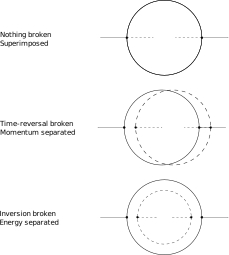
\includegraphics[width=0.75\textwidth]{figures/spinStructureWeyl}
  \caption{\label{fig:spinStructure} }
\end{figure}



\subsection{Symmetries}
In order to separate weyl cones in momentum, we introduce a pseuod spin degree of freedom, making the system 4x4.
We may then get solutions with the cones separated in momentum (or energy).
We may also ask what heppens if we try to separate tilted cones?

Firstly, in the most intuitive way to extend the 2x2 tilted cones to 4x4, we get that the cones tilt opposite direction, thus not superimposed even before separating in momentum.
They are after that simple to separate in momentum.
We might wonder if it makes sense to do it in this way.

The lattice model of the energy dispersion to explain tilted cones gives two cones separated in momentum, and tilting corresponds to ``bending'' the dispersion curves between them.
Maybe we therefore always have cones separated in momentum, and thus tilting superimposed does not make sense?
All depends on the origin of the tilt I believe.
Also, we must not confuse the global dispersion relation, to the Dirac cones which are expansions around the nodes.

Key to understand how spin behaves in all of this, and also maybe the symmetries.

To properly investigate the symmetry properties of the system, we must consider the 4x4, not 2x2 Hamiltonians.
While the 2x2 system does a goood job at describing a single cone, much important phsycis is lost when reducing the 4x4 Hamiltonian.
For example, the requirement that the total Berry curvature over the entire Briolluine zone is zero is not met for the 2x2 Hamiltonian, as it describes only one cone of a certain chirality.
The 4x4, however, includes two cones, which may in general be superimposed, thus conserving the total zero-divergence of the Berry curvature.
As a matter of fact, the inclusion of both cones is important also for symmetry considerations.

Let
\[
  H = v_{F} \tau _{x} \otimes \vec{\sigma} \vec{k},
\]
where \(\tau \) is some pseudo spin degree of freedom, transforming like \(\vec{r}\) under parity in time reversal.
This system describes two superimposed cones at the origin, with opposite chirality.
The effect of parity \(\mathcal{P}\) and time reversal \(\mathcal{T}\) is
\begin{table}[h]
  \centering
  \begin{tabular}{lcc}
    & \(\mathcal{P}\) & \(\mathcal{T}\)\\
    \hline
    \(\tau \) & - & +\\
    \(\sigma \) & + & -\\
    \(k\) & - & -
  \end{tabular}
\end{table}
\begin{equation}
  \label{eq:111}
  \begin{aligned}
    \mathcal{P} \tau \mathcal{P}^{\dagger} &= -\tau, & \mathcal{T} \tau \mathcal{T}^{\dagger} &= +\tau\\
    \mathcal{P} \sigma  \mathcal{P}^{\dagger} &= + \sigma,  & \mathcal{T} \sigma  \mathcal{T}^{\dagger} &= -\sigma \\
    \mathcal{P} k \mathcal{P}^{\dagger} &= -k, & \mathcal{T} k \mathcal{T}^{\dagger} &= -k
  \end{aligned}
\end{equation}
Obviously then, the Hamiltonian is both time reversal and parity invariant, as \(\mathcal{P} \mathcal{P}^{\dagger} = \mathcal{T} \mathcal{T}^{\dagger} = 1\).

A tilt term \(\tau _{x} \otimes \mathcal{I} \vec{\omega} _{0} \vec{k}\) breaks time reversal invariance, while maintaining parity invariance.
This is due to the two cones of opposite chirality tilting in opposite directions.

\begin{figure}[h]
  \centering
  \tikzsetnextfilename{symmetryspin}
  \begin{tikzpicture}
    \draw[->] (-4, 0) -- (4, 0) node[right] {\(k\)};
    \draw[->] (0, 0) -- (0, 4) node[right] {\(E\)};

    % vf = 1, v0 = 0.8
    \draw[blue] (-3.5, 0.7) -- (0, 0) -- (2, 3.6) node[right] {\(\ket{\uparrow}\)} coordinate[pos=0.7] (a);
    \draw[red] (3.5, 0.7) node[right] {\(\ket{\downarrow }\)} -- (0, 0) -- (-2, 3.6)
    coordinate[pos=0.7] (b);

    \draw[->] (a) -- ++(1, 0);
    \draw[->] (b) -- ++(1, 0);
  \end{tikzpicture}
  \caption{Time reversal breaking in tilted system.
    Cross section in the tilt direction shown, with blue showing one cone and red the other.
    Black arrows indicate spin direction, which for \(\ket{\uparrow {}}\) is proporitional to  \(k\) while for \(\ket{\downarrow {}}\) is proportional to \( -k \).
  }
\end{figure}

The unperturbed Dirac Hamiltonian is Lorentz invariant, given that we consider an ``effective speed of light'', namely the Fermi velocity, instead of the actual speed of light \( c \).
Specifically, Lorentz invariance means invariance under the \emph{Lorentz group}.
The Lorentz group is the \( O(1,3) \) Lie group that conserves
\[
x_{\mu } x^{\mu } = t^2 - x^2 - y^2 - z^2,
\]
i.e. all isometries of Minkowski space.
More specifically, the group consists of all 3D rotations, \( O(3) \), and all \emph{boosts}.
A boost is a hyperbolic rotation from a spactial dimension to the temporal dimension.
If we now direct our focus at the Hamiltonian of the Dirac cone
\[
H = \pm v_{F} \vec{\sigma} \vec{p},
\]
we may easily show the Lorentz invariance of the system.
The time independent Schrodinger equation is
\begin{equation}
  \label{eq:112}
  H \ket{\psi } = E \ket{\psi } \implies (H^2 - E^2) \ket{\psi } = 0.
\end{equation}
As
\[
p^{\mu } = \left(\frac{E}{c}, \vec{p}\right),
\]
the operator in Eq. \eqref{eq:112} is nothing more than
\todo{ Make clear the matrix strucute here. There is an implicit identity matrix of size 2 }
\begin{equation}
  \label{eq:113}
  H^2-E^2 = v_{F}^2 \vec{p}^2 - c^2 \left(p^0\right)^2 ,
\end{equation}
where we used the anticommutation relation
\[
\{\sigma_{i}, \sigma_{j}\} =  2 \delta _{ij}
\]
of the Pauli matrices.
Using now the effective speed of light \( c=v_F \), Eq. \eqref{eq:113} is
\begin{equation}
  \label{eq:114}
  - v_F^2 p_{\mu } p^{\mu }.
\end{equation}
The invariance of \( x^{\mu} x_{\nu} \) is the very definition of the Lorentz group, and so is obviously Lorentz invariant.

Consider now a \emph{tilted} Dirac cone
\begin{equation}
  \label{eq:115}
  H = \pm v_F \vec{\sigma} \vec{p} + \omega_x k_x,
\end{equation}
where we, without loss of generality, chose the tilt to be in the \( x \)-direction.
By the same argumentation as above, the eigenequation
\[
  H \ket{\psi} = E\ket{\psi} \implies (H^2 - E^2)\ket{\psi} = 0
\]
leads to the equation
\begin{equation}
  \label{eq:116}
  -v_F^2 p^{\mu} p_{\mu} + \omega_{x} k_x (2 E - \omega_x k_x) = 0.
\end{equation}
This is \emph{not} invariant under a Lorentz transformation, as can be seen by, for example, a rotation around the \( z \)-axis.
\todo{Clean up p vs k}



